% Options for packages loaded elsewhere
\PassOptionsToPackage{unicode}{hyperref}
\PassOptionsToPackage{hyphens}{url}
\PassOptionsToPackage{dvipsnames,svgnames,x11names}{xcolor}
%
\documentclass[
  12pt,
]{article}
\usepackage{amsmath,amssymb}
\usepackage{iftex}
\ifPDFTeX
  \usepackage[T2A]{fontenc}
  \usepackage[utf8]{inputenc}
  \usepackage{textcomp} % provide euro and other symbols
\else % if luatex or xetex
  \usepackage{unicode-math} % this also loads fontspec
  \defaultfontfeatures{Scale=MatchLowercase}
  \defaultfontfeatures[\rmfamily]{Ligatures=TeX,Scale=1}
\fi
\usepackage{lmodern}
\ifPDFTeX\else
  % xetex/luatex font selection
  \setmainfont[]{Linux Libertine}
  \setmonofont[]{Liberation Mono}
\fi
% Use upquote if available, for straight quotes in verbatim environments
\IfFileExists{upquote.sty}{\usepackage{upquote}}{}
\IfFileExists{microtype.sty}{% use microtype if available
  \usepackage[]{microtype}
  \UseMicrotypeSet[protrusion]{basicmath} % disable protrusion for tt fonts
}{}
\makeatletter
\@ifundefined{KOMAClassName}{% if non-KOMA class
  \IfFileExists{parskip.sty}{%
    \usepackage{parskip}
  }{% else
    \setlength{\parindent}{0pt}
    \setlength{\parskip}{6pt plus 2pt minus 1pt}}
}{% if KOMA class
  \KOMAoptions{parskip=half}}
\makeatother
\usepackage{xcolor}
\usepackage[a4paper,margin=2cm]{geometry}
\usepackage{graphicx}
\makeatletter
\def\maxwidth{\ifdim\Gin@nat@width>\linewidth\linewidth\else\Gin@nat@width\fi}
\def\maxheight{\ifdim\Gin@nat@height>\textheight\textheight\else\Gin@nat@height\fi}
\makeatother
% Scale images if necessary, so that they will not overflow the page
% margins by default, and it is still possible to overwrite the defaults
% using explicit options in \includegraphics[width, height, ...]{}
\setkeys{Gin}{width=\maxwidth,height=\maxheight,keepaspectratio}
% Set default figure placement to htbp
\makeatletter
\def\fps@figure{htbp}
\makeatother
\setlength{\emergencystretch}{3em} % prevent overfull lines
\providecommand{\tightlist}{%
  \setlength{\itemsep}{0pt}\setlength{\parskip}{0pt}}
\setcounter{secnumdepth}{-\maxdimen} % remove section numbering
\ifLuaTeX
\usepackage[bidi=basic]{babel}
\else
\usepackage[bidi=default]{babel}
\fi
\babelprovide[main,import]{ukrainian}
\ifPDFTeX
\else
\babelfont[ukrainian]{rm}{Linux Libertine}
\fi
% get rid of language-specific shorthands (see #6817):
\let\LanguageShortHands\languageshorthands
\def\languageshorthands#1{}
\ifLuaTeX
  \usepackage{selnolig}  % disable illegal ligatures
\fi
\IfFileExists{bookmark.sty}{\usepackage{bookmark}}{\usepackage{hyperref}}
\IfFileExists{xurl.sty}{\usepackage{xurl}}{} % add URL line breaks if available
\urlstyle{same}
\hypersetup{
  pdflang={uk-UA},
  colorlinks=true,
  linkcolor={blue},
  filecolor={Maroon},
  citecolor={Blue},
  urlcolor={Blue},
  pdfcreator={LaTeX via pandoc}}

\author{}
\date{}

\begin{document}

\hypertarget{radians}{%
\section{Radians}\label{radians}}

Sine is defined in terms of radians as

\[
sin(x) = x - \frac{x^3}{3!} + \frac{x^5}{5!} - \frac{x^7}{7!}
\]

This formula only works when x is in radians! Why? Well, sine is
fundamentally related to distance moved, not head-tilting. But we'll
save that discussion for another day.

\hypertarget{the-wheels-are-turning-2000-degrees-per-second.-youd-think}{%
\subsubsection{``The wheels are turning 2000 degrees per second''. You'd
think:}\label{the-wheels-are-turning-2000-degrees-per-second.-youd-think}}

\begin{quote}
Ok, the wheels are going 2000 degrees per second. That means it's
turning 2000/360 or 5 and 5/9ths rotations per second. Circumference = 2
* pi * r, so it's moving, um, 2 * 3.14 * 5 and 5/9ths\ldots{} where's my
calculator\ldots{}
\end{quote}

\hypertarget{ok.-now-imagine-a-car-with-wheels-of-radius-2-meters-also-a-monster.-the-car-wheels-are-turning-6-radians-per-second.-youd-think}{%
\subsubsection{Ok. Now imagine a car with wheels of radius 2 meters
(also a monster). ``The car wheels are turning 6 radians per second''.
You'd
think:}\label{ok.-now-imagine-a-car-with-wheels-of-radius-2-meters-also-a-monster.-the-car-wheels-are-turning-6-radians-per-second.-youd-think}}

\begin{quote}
Radians are distance along a unit circle --- we just scale by the real
radius to see how far we've gone. 6 * 2 = 12 meters per second. Next
question.
\end{quote}

\hypertarget{section}{%
\subsection{\ldots{}}\label{section}}

Radians to the rescue! Knowing they refer to distance traveled (they're
not just a ratio!), we can interpret the equation this way:

\begin{enumerate}
\def\labelenumi{\arabic{enumi}.}
\tightlist
\item
  x is how far you traveled along a circle
\item
  sin(x) is how high on the circle you are
\end{enumerate}

\begin{figure}
\centering
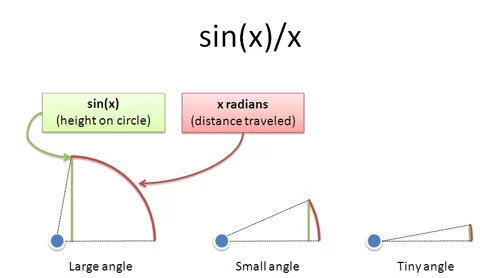
\includegraphics{sinx.png}
\caption{qwrou}
\end{figure}

When something moves a tiny amount, such as 0 to 1 degree from our
perspective, it's basically going straight up. If you go an even smaller
amount, from 0 to .00001 degrees, it's really going straight up. The
distance traveled (x) is very close to the height (sin(x)).

As x shrinks, the ratio gets closer to 100\% --- more motion is straight
up. Radians help us see, intuitively, why sin(x)/x approaches 1 as x
gets tiny. We're just nudging along a tiny amount in a vertical
direction. By the way, this also explains why sin(x) \textasciitilde{} x
for small numbers.

Sure, you can rigorously prove this using calculus, but the radian
intuition helps you understand it.

Remember, these relationships only work when measuring angles with
radians. With degrees, you're comparing your height on a circle (sin(x))
with how far some observer tilted their head (x degrees), and it gets
ugly fast.

\end{document}
